\section{Software Diversity}

Software diversity is the study of diversity in software and software engineering. It is
a diverse discipline and there is a wide range of research all with different focus and
set of goals. The one common factor is that they all explore the potential benefits of
diverse engineering \cite{survey}.

Software diversity has a myriad of applications ranging from fault-tolerance to re-usability
to security \cite{survey}. For security puposes it is a relatively common approach to
certain issues such as memory error exploits and different approaches have been taken.
For example \textcite{os-randomization} randomizes the interface between user space
applications and the operating system, \textcite{mem-exploits} introduces a level of
indirection to function call to randomize static data at the C source code level and
\textcite{add-obfuscation} obfuscates the code and data of an executable by randomizing
the absolute locations.
% Stuff about memory errors
% \cite{os-randomization,mem-exploits,add-obfuscation,compiler-generated-sw-div}

Failing to defend against certain memory errors can introduce new attack vectors for a
determined adversary. Some of these attacks are based on the availability to reverse engineer
a vulnerable executable, where software diversity can once again prove an effective defense.
To defend against reverse-engineering based attacks \textcite{binary-stirring} dynamically
determine the addresses of basic blocks at load time, \textcite{smashing-gadgets} performs
in-place code randomization to make each executable look different without incurring
significant overhead and \textcite{librando} implements a library to transparently
diversify code compiled and executed by JIT-compilers.

Many more strategies and techniques exist for what is known as
\textit{automated software diversity} and \textcite{SoK} provides an overview of different
goals, attacks, defenses and deployment methods. \textit{Automated} refers to the fact that
a human is not involved in the process (other than devising the process).

% Stuff about ROP and other reverse engineering, code re-use attacks
%\cite{SoK,binary-stirring,large-scale-automated,readactor,smashing-gadgets,synthetic-diversity,librando},

What all of these techniques have in common is that they introduce some kind of chance into
the development toolchain, which as mentioned will not be the approach taken in this paper.
Instead the focus will be on systematic and deterministic generation of \textit{static}
diversity.  Static diversity entails generating several, diverse executables; In contrast
to \textit{dynamic} diversity which involves providing diverse run-times\cite{survey}.

The motivation is that by employing diversification techniques one can break the
reactive nature of software security and shift the advantage from the attacker to the
defender \cite{compiler-generated-sw-div}.

\subsection{Return Oriented Programming}
\label{rop}

\textcite{rop} introduces \textit{return-oriented programming} (ROP) as an extension of
the \textit{return-to-libc}\cite{return-into-libc} attack that allows arbitrary code
execution without the limitation of calling complete functions. All examples in this
subsection is only concerned with the x86 and x86-64 architecture.

A typical return-into-libc attack involves somehow diverting the program control
flow to transfer control to code that already exists in the program's address space,
it could e.g be the system() library function, and use it in an unintended manner. For
example an adversary could utilize a buffer overflow to overwrite the return address on
the stack so that it instead points to a function call that leaks sensitive information.
By first jumping to a sequence of instructions such as "pop reg; pop reg; ret;" it is
possible to chain together several of these function calls, performing more complex
operations \cite{non-exec-stack,advanced-return-into-libc}.

\textcite{rop} builds upon this concept by instead diverting the control flow to just these
short sequences of instructions, usually just two or three instructions, typically ending
with a "ret" instruction. These sequences are dubbed \textit{gadgets} and by carefully
choosing and chaining them together one can achieve arbitrary code execution \cite{rop}.

For instruction set architectures with varying instruction sizes there can be gadgets not
explicitly placed there by the compiler. \textcite{rop} explains them with an analogy to
the English language; Where the word "dress" can be found in "Address" and the word "head"
can be found in "The Address" depending on where you start and stop reading. When
instructions can be of varying lengths then the same sequence of bytes can be interpreted
as different instructions depending on where one starts reading. If you can find a hidden
"ret" instruction you can potentially find a whole gadget not explicitly placed there by
the compiler.

The reason that the "ret" instrution is convenient is because it transfers control flow
to the instruction pointed to by the value at the top of the stack. I.e the "ret" instruction
reads the top of the stack as a memory address and transfers the control flow to continue
from that address. If an adversary can control the stack he or she can also control the
control flow. Gadgets can end with other instructions depending on what is desirable.

\subsubsection{A return-into-libc/ROP-attack Example}

As an example attack consider the x86-64 version of the "split" challenge on ROP emporium
\footnote{https://ropemporium.com/challenge/split.html}. The challenge consists of two
files, a binary that is vulnerable to a buffer overflow and a "flag.txt" file. The goal
is to provide a payload to the stdin of the binary that executes the command
"/bin/cat flag.txt". It is a simple challenge in the sense that the string "/bin/cat flag.txt"
and a call to the \textit{system()} function (which executes a shell command) are already
present in the binary.

In order to call the \textit{system()} function in an unindented manner we can exploit
the buffer overflow vulnerability. Specifically in this example, the vulnerability is that
a buffer of size 32 bytes is allocated and 92 bytes is read into it. The string will grow
from lower memory addresses to higher while the stack grows from higher addresses to
lower. In other words, by writing 92 bytes to the buffer, the top 60 bytes of the stack
will be overwritten. Included in these 60 bytes is the \textit{return address} and by
overwriting this to the location of the \textit{system()} function call we can call the
function in an unindented manner.

The calling convention of the AMD64 Linux Kernel is to load the arguments to the kernel
interface in registers \textit{rdi, rsi, rdx, r10, r8 and r9} in that order\cite{system-v-abi}.
In other words, we want the \textit{rdi} register to point to the "/bin/cat flag.txt" string
before we call the \textit{system()} function. In order to do this we must find the sequence
"pop rdi; ret" somewhere in the binary. If we manage to execute this gadget when the
address of the "/bin/cat flag.txt" is at the top of the stack and the address of the call to
\textit{system()} is at the penultimate position the "pop rdi" instruction will load the
address of the argument into the rdi register and increment the stack pointer (remember
that the stack grows downwards). The "ret" instruction will then read the now current
value at the top of the stack, which is the address to the \textit{system()} call, and
transfer the program control there.

Putting this together, we want to overwrite the return address of the vulnerable function
with the address of our gadget (i.e the address of the "pop rdi" instruction). When control
is transfered to the gadget the top of the stack should be the address of the "/bin/cat flag.txt"
string, followed by the address of the \textit{system()} call.

To find the offset of the return address we can run the program in a debugger and enter
garbage to the stdin, e.g "AAAABBBBCCCCDDDDEEEEFFFF" and so on. If we overwrite the return
address the program will most likely raise a segmentation fault, and from the core dump we
can read what address it tried to divert control flow to. If it is e.g "0x45454545" (which
is the ascii encoding of "EEEE") we know that by padding our payload with 16 characters we
overwrite the return address. There are more clever ways to do this but the simple way
also work. In this case the padding required is 40 bytes.

The address of the gadget (the "pop rdi" instruction) to be used is 0x400883, the address
of the "/bin/cat flag.txt" string is 0x601060 and the address of the system call is
0x400810. All of these addresses as well as the required padding were found using the
radare2\footnote{https://github.com/radare/radare2} utility. We want to place the address
of the gadget at the return address, followed by the address of the "/bin/cat flag.txt"
followed by the address of the system call. We know from forcing a segmentation fault that
to overwrite the return address we need 40 bytes of padding. We also know that since the
input buffer and the stack grows in different directions the stack will read our values in
the order we write them.

The hexadecimal encoded payload for this example is thus:

\seqsplit{41414141414141414141414141414141414141414141414141414141414141414141414141414141830840000000000060106000000000001008400000000000}

which includes 40 "A"s (0x41) as padding, followed by the little endian
representation of the addresses, each of which is 8 bytes (16 hexadecimal digits). When
this payload is posted the stack will look like Figure \ref{fig:after-payload}.

\begin{figure}[h]
	\centering
	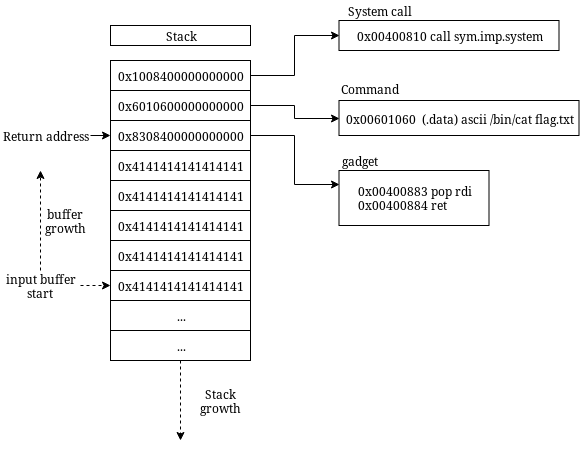
\includegraphics[width=\textwidth]{background/software-diversity/figures/after-payload}
	\caption{The contents of the stack and pointer references after the payload has been posted.}
	\label{fig:after-payload}
\end{figure}

The function requesting the input will reach its "ret" instruction, 0x400883 will be popped
from the stack and the control flow will be transfered there. The stack will now look like
presented in Figure \ref{fig:after-first}.

\begin{figure}[h]
	\centering
	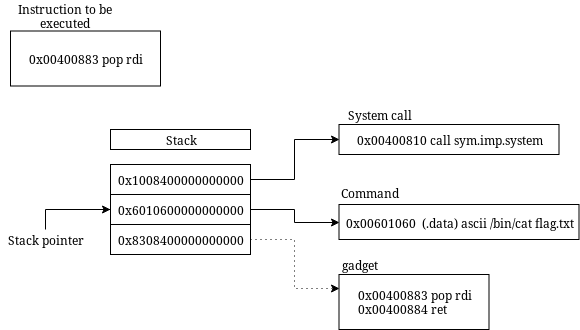
\includegraphics[width=\textwidth]{background/software-diversity/figures/after-first}
	\caption{The contents of the stack, the stack pointer and pointer references after the first ret instruction.}
	\label{fig:after-first}
\end{figure}

The "pop rdi" instruction will be executed and 0x601060 will be loaded into register rdi
and the stack pointer is incremented. 0x400810 is now at the top of the stack and when the
following ret instruction is executed the control flow will be transfered to the
instruction at address 0x400810, which is a call to the system function (see Figure
\ref{fig:after-second}).

\begin{figure}[h]
	\centering
	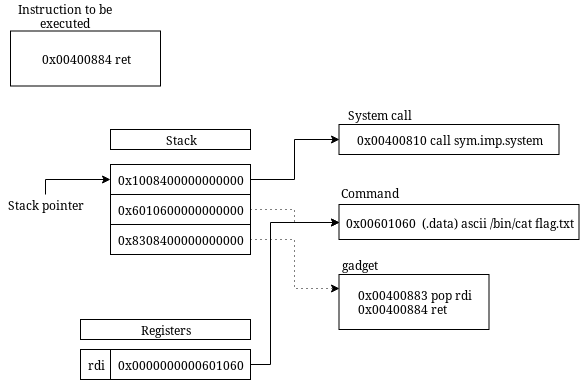
\includegraphics[width=\textwidth]{background/software-diversity/figures/after-second}
	\caption{The contents of the stack, the stack pointer, pointer references and contents of the rdi register after the second ret instruction.}
	\label{fig:after-second}
\end{figure}

The system function, whose argument is located in the rdi register, will read the
"/bin/cat flag.txt" string and execute the command and the contents of flag.txt will be
printed.

Appendix \ref{appendix:rop-exploit} contains the source code of a python script that
executes this attack.

This "attack" does not actually do anything malicious, as it is just an example. As mentioned
it was also fairly simple in the sense that the argument to be passed to \textit{system()}
was already present in the binary. One could supply this argument with the payload. In
fact, including a "/bin/sh" string in the payload and providing it as an argument to the
\textit{execve()} function is one of the examples described by \textcite{rop} when
introducing the return oriented programming concept. In this example \textcite{rop} performs
a number of computations to set up the arguments, showing that if one is clever enough
there are few limits to what code can be executed simply be re-using the code already
present in the binary.

\subsubsection{Defending against return-into-libc/ROP-attacks}

Defending against a technique such as the one exemplified above is difficult. Gadgets will
always be present in every binary. But as mentioned software diversity can provide some
manner of protection. The idea is that since an adversary is reliant of the exact
addresses of these gadgets a way to limit the possible attack surface is by creating a
population of binaries who share as few of these gadgets as possible, and then distribute
these evenly among all users. An adversary would then have to identify which version the
target is running, obtain and analyze that version and create a tailored payload. This
payload can then \textit{not} be re-used on any other version of this program.

For example, the payload crafted for the example above only works on that binary. If a
compiler could generate two binaries, the one "attacked" above and one where the
\textit{system()} call is shifted to the address 0x00400808. I would have to create a new,
different payload for the latter binary since the payload crafted above would not work if
the \textit{system()} call is not located at 0x00400810. In fact, the payload crafted in
the example would not work if the address of the gadget, the system call \textit{or} the
address of the command string changed.
